% This is based on "sig-alternate.tex" V1.9 April 2009
% This file should be compiled with V2.4 of "sig-alternate.cls" April 2009
%
\documentclass{report}

\usepackage[english]{babel}
\usepackage{graphicx}
\usepackage{tabularx}
\usepackage{subfigure}
\usepackage{enumitem}
\usepackage{url}


\usepackage{color}
\definecolor{orange}{rgb}{1,0.5,0}
\definecolor{lightgray}{rgb}{.9,.9,.9}
\definecolor{java_keyword}{rgb}{0.37, 0.08, 0.25}
\definecolor{java_string}{rgb}{0.06, 0.10, 0.98}
\definecolor{java_comment}{rgb}{0.12, 0.38, 0.18}
\definecolor{java_doc}{rgb}{0.25,0.35,0.75}

% code listings

\usepackage{listings}
\lstloadlanguages{Java}
\lstset{
	language=Java,
	basicstyle=\scriptsize\ttfamily,
	backgroundcolor=\color{lightgray},
	keywordstyle=\color{java_keyword}\bfseries,
	stringstyle=\color{java_string},
	commentstyle=\color{java_comment},
	morecomment=[s][\color{java_doc}]{/**}{*/},
	tabsize=2,
	showtabs=false,
	extendedchars=true,
	showstringspaces=false,
	showspaces=false,
	breaklines=true,
	numbers=left,
	numberstyle=\tiny,
	numbersep=6pt,
	xleftmargin=3pt,
	xrightmargin=3pt,
	framexleftmargin=3pt,
	framexrightmargin=3pt,
	captionpos=b
}

% Disable single lines at the start of a paragraph (Schusterjungen)

\clubpenalty = 10000

% Disable single lines at the end of a paragraph (Hurenkinder)

\widowpenalty = 10000
\displaywidowpenalty = 10000
 
% allows for colored, easy-to-find todos

\newcommand{\todo}[1]{\textsf{\textbf{\textcolor{orange}{[[#1]]}}}}

% consistent references: use these instead of \label and \ref

\newcommand{\lsec}[1]{\label{sec:#1}}
\newcommand{\lssec}[1]{\label{ssec:#1}}
\newcommand{\lfig}[1]{\label{fig:#1}}
\newcommand{\ltab}[1]{\label{tab:#1}}
\newcommand{\rsec}[1]{Section~\ref{sec:#1}}
\newcommand{\rssec}[1]{Section~\ref{ssec:#1}}
\newcommand{\rfig}[1]{Figure~\ref{fig:#1}}
\newcommand{\rtab}[1]{Table~\ref{tab:#1}}
\newcommand{\rlst}[1]{Listing~\ref{#1}}

% General information

\title{Ripple BT - The future of local social networking\\
\normalsize{Distributed Systems -- Project Proposal}}
\subtitle{subtitle}

% Use the \alignauthor commands to handle the names
% and affiliations for an 'aesthetic maximum' of six authors.

\numberofauthors{1} %  in this sample file, there are a *total*
% of EIGHT authors. SIX appear on the 'first-page' (for formatting
% reasons) and the remaining two appear in the \additionalauthors section.
%
\author{
% You can go ahead and credit any number of authors here,
% e.g. one 'row of three' or two rows (consisting of one row of three
% and a second row of one, two or three).
%
% The command \alignauthor (no curly braces needed) should
% precede each author name, affiliation/snail-mail address and
% e-mail address. Additionally, tag each line of
% affiliation/address with \affaddr, and tag the
% e-mail address with \email.
%
% 1st. author
\alignauthor \normalsize{Carl Friess, Isaak Hanimann, Sven Knobloch, Laurin Paech,  Sebastian Winberg, David Yenicelik}\\
	\affaddr{\normalsize{cfriess  15-943-111, isaakh 15-913-312, knsven 14-945-166, lpaech 15-944-242, winbergs 15-941-222,  yedavid 15-944-366}}\\
	\email{\normalsize{cfriess@student.ethz.ch, isaakh@student.ethz.ch, knsven@student.ethz.ch, lpaech@student.ethz.ch, winbergs@student.ethz.ch, yedavid@student.ethz.ch}}
}


\begin{document}

\maketitle

\begin{abstract}
We propose a social networking application for sharing photos in close physical proximity. 
A user can take a picture, which is then broadcasted to all phones that are in the direct vicinity and part of the network. \\
To increase speed and reduce operating costs, the Android application does not solely rely on high-bandwidth connections with a centralized server, but rather uses a distributed peer to peer network to transmit photos between individual nodes.
Our proposed app utilizes a combination of the Bluetooth Low Energy and BitTorrent protocols, as well as a custom RESTful HTTP API.\\
The fundamental transfer of image files is done using BitTorrent. A central tracker will facilitate the discovery of nodes in accordance with the BitTorrent protocol. A receiving node will then download the image form the initial node and from other nodes, which have already completed the download. The tracker will use a JavaScript BitTorrent implementation \todo{Link} executed in a node.js environment hosted on a AWS EC2 instance.\\
Devices use the Bluetooth Low Energy Protocol for close proximity device discovery and for transmitting identifying information of  the broadcasted images.\\
A centralized server further allows devices to retrieve torrent files, which are necessary for the BitTorrent protocol.\\
Our goal is to have a fully-working prototype with the proposed architecture.
All participating, delivering and receiving nodes are determined by the tracker.
\end{abstract}

\section{Introduction}

We first introduce a few definitions.

\begin{enumerate}
\item \textbf{ripple} \textit{(noun)}: A photo that is being shared with anyone nearby from a central person's smartphone. We will use the words 'ripple' and 'photo' interchangeably. 
\item \textbf{to ripple} \textit{(verb)}: When person A shares a photo (the ripple), and person B decides to share it again, the photo has 'rippled' once as it propagated over one person since the initial share.
\item \textbf{tracker}: A central server handling the distribution logic
\item \textbf{AWS}: Amazon Web Services. The cloud, which will act as the tracker.
\item \textbf{P2P}: Peer to peer
\item \textbf{$ n $}: The number of nodes in observed network. In our case, these nodes will be android devices.
\end{enumerate}

\subsection{Problem Statement and Motivation}
There are numerous social networks, such as Instagram and Snapchat, allowing users to share moments with a specific group of people.
These services are often criticized for removing the personal element from social communication, because users are sitting behind screens or using their phones, rather than actually spending time together.\\
Our approach to social networking is to augment social interaction, rather than redefining and possibly inhibiting it. Social Networks should help form connections between people and not just build on existing ones.

\subsection{Concept}
Considering the above problem statement, we propose Ripple: a social network allowing users to share moments with other users in their close proximity. The social network will consist of a freely available Android application with a focus on photos.\\
After a user takes a picture it is broadcasted to all other users of the app in their immediate vicinity, regardless of their affiliation with the broadcasting user. Communication is in principle anonymous (disregarding content) and always public.\\
Users receiving brodcasted images may view them once. They are then presented with the choice of either simply discarding the image or instead rebroadcasting ('re-rippling') it to other users in their proximity.
Each user can view the ripple only once regardless of the number of re-ripples near them.\\
We believe this social network will encourage social interaction, as the communication can only take place when users are close to each other. Furthermore, the network allows interesting content to 'propagate', making it possible to share memorable moments in a wider radius.

\subsection{Application Scenario}
We will demonstrate a typical use case of the Android application in a group of people attending an event: \textit{Alice}, \textit{Bob}, \textit{Charlie} and \textit{Daniel}.\\
Alice takes a funny photo of a particular activity at the event and wants to raise awareness of the activity with other attendees. She therefore uses Ripple to share the image.\\
Bob, who is not far away receives the ripple and is intrigued by the picture. He thinks others might share his intrigue and re-ripples the image.\\
Charlie and Daniel are in close proximity of Bob but not of Alice. As Bob is also broadcasting the image and they have the Ripple app installed, they now also receive the ripple.\\
Following this scheme the ripple spreads out and propagates, maybe even beyond the event's location.

\subsection{Background}
This concept is related to an iOS application developed at the START Hack hackathon in March 2017. It is a basic implementation of this concept using Amazon S3 to store images, so they can be downloaded by the receiving devices. Bluetooth Low Energy is used to advertise images by setting the value of a well known GATT characteristic to the UUID of the image in the S3 bucket.\\
While this implementation works, it has several flaws. Firstly, uploading every image to an Amazon S3 bucket means that operation costs for storage are bound to be high without heavy compression, leading to low quality content.\\
Similarly, repeatedly downloading the image from one central point, causes high bandwidth consumption and possibly unnecessary data transfer costs.\\
Beyond this, the method for announcing ripples is also suboptimal. It does not work well, when a user would like to broadcast multiple ripples in quick succession and (on iOS) does not fully work when the application is in the background.\\
With Ripple BT we aim to redesign the system from the ground up with a focus on spreading the load of sending images among user devices, thus reducing operating costs and improving performance.

\subsection{Challenges}
This project has two main distributed challenges:
\begin{enumerate} 
    \item Finding users in close proximity
    \item Sending the image data
\end{enumerate}

For the first challenge of user discovery we investigated using GPS data to track the user location. Since GPS has a fairly weak accuarcy with uncertanties as high as a few hundred meters when inside a building, we couldn't achieve sufficient locality using this technology. We therefore turned our focus to Bluetooth Low Energy. The range of 10-20 meters is optimal considering the desired behavior and less power consuming than GPS. Furthermore Bluetooth Low Energy provides a well established protocol with wide-spread hardware compatibility.

We considered the following aspects for the second challenge of sending the image data.
It became clear early on that Bluetooth Low Energy would not have high enough data rates to send an entire image from one device to another in a reasonable time frame and acceptable reliability. For this reason we first looked into a centralized structure (using Amazon S3) where images are stored with a UUID and the UUID is sent to the receiver over Bluetooth. The image can then be retreived from the central server using the UUID.

While this implementation works, storage and bandwidth costs especially for a later support of video files would be fairly high. With the intentions of shifting most of the load to user devices and not storing the image data on a central server we looked into peer to peer technology. We considered the use of IPFS but decided to use the BitTorrent file sharing protocol since it is well established and commonly used with a large amount of software support. \todo{java librabry} 

With BitTorrent the devices can distribute the content between themselves. However, this requires a torrent file, leading to the question of how to send this file to other devices. Our first idea was to send the torrent file over Bluetooth Low Energy. But since torrent files can have a significant size themselves and BLE only allows for low data rates, we chose to only pass an identifier over Bluetooth and retreive the torrent file from the central server  using a custom RESTful HTTP API. Since one torrent file is only a few kilobytes big, we have significantly lowered the cost by several orders of magnitude.


\section{System Overview}


\subsection{System Architecture}
We describe the distributed system architecture with regards to the above presented challenges. \\

We intend to solve 1.) by a \textit{P2P} (peer to peer) network which makes a central server redundant.
Instead of downloading all photos from a central server, each phone is a node and independently transmits it's captured image directly to it's close neighbours. 
It also has the benefit that we remove any single point of failure within the system, as there are multiple possible paths to a receiver from a sender in the network of phone-nodes (assuming multiple people are in physical proximity to the sender and the receiver). 
We must handle some logic tasks though, for which we use a central server through \textit{AWS} (Amazon Web Services), which decides which phone should receive which photos, and which other nodes to contact for this data. 
It is important to emphasis that there are no photos saved on the server, and as such, no major load to be handled uploading and downloading.
This effectively solves the problem of data-congestion in a single point, and reduces points of failures. 

Challenge 3.) can  be solved by using dynamic algorithms that work on the position of a user. 
However, for this project, we assume that we are in a network where more than 5 people are in physical proximity, making any technology a viable option for distribution of the photos.
\newline
P2P technology has been used extensively in torrenting applications, and has proven to work reliably and efficiently. 
As such, we assume that it proposes a highly-scalable technology with the ability to be rapidly deployable and efficient-to-run with regards to our application scenario.
Our proposed system architecture is a well-established solution in a novel setting.
Conventional P2P don't use mobile devices but stationary, reliably and well-connected agents. 
Our system architecture is simple, as we will use one central \textbf{tracker}, which will handle the distribution and communication logic of the photos and nodes, and $ n $ number of \textbf{nodes}, which will form the phones that can upload and receive the pictures.
We use a tracker instead of distributed hash table (DHT) to improve the speed of peer discovery and lower the overhead.

\subsection{Distribution of Torrent Files}
One of the challenges that we face is the limited data rates using BLE.
That leads to the issue that we can't distribute the torrent files via BLE but instead we use a Server that distributes the torrent files to nodes that request them by sending a UUID of a picture. \newline
Node A sends the UUID to Node B after uploading it to the server and notifying the tracker of a new file. 
Node B requests the torrent file by sending the UUID to the server.
The server verifies the UUID by look up in a database, retrieving the corresponding torrent and sending it to Node B. Node B can now use the torrent file to download the picture over the BitTorrent Protocol by contacting the Tracker, which provides a list of seeds.

\subsection{Bluetooth Low Energy}
For the Bluetooth Low Energy we have come up with the following protocol: 
Each device will have a well known GATT service for Ripples. In this service there is a well known characterisitic that stores a sequence number. In addition, the service will have a characteristic for each Ripple it is currently advertising. The UUID of that characteristic is used for querying the torrent file from the central server.

The device is constantly scanning for devices with the Ripple GATT service and connects to them automatically.

If a device wants to send/broadcast a Ripple, it adds a characteristic with the respective UUID to the Ripple GATT service and increments the value of the sequence number characteristic. This will notify connected devices of potential changes and the existance of a new Ripple. The receiving device will then scan for new characteristics and continue to retreiving the image for the Ripple.


\subsection{Components}
Given the above system architecture, we have two components. 

\begin{enumerate}
\item \textbf{Tracker:} Handles the distribution logic of the photos, without storing the pictures. 
Only IP, location, permissions etc. are uploaded and downloaded from the server, allowing this to have a low worst-case and average load. 
\item \textbf{Nodes:} Are the phones that receive the photos. 
%%DESCRIBE WHICH PROTOCOLS TO USE
These nodes communicate with each other using over simple internet protocols, and are responsible for sharing the files. As such, the load is taken away from the cloud. 
This also makes the network more reliable and fast. There is no single point of failure, and one phone can receive small data-packets (which combined forms a picture) from multiple other phones that can provide the data packets.
\end{enumerate}

\begin{figure}[h]
	\centering
    \includegraphics[width=\columnwidth]{rippleslide.png}
    \lfig{example}
    \vspace{-5mm} % use negative white space to fix too large gaps
	\caption{What our final product could look like. Includes a view to take photos (left), a list of all received and opened photos (middle), and a screenshot of what a photo looks like right after when it's taken and before it's shared (right)}
\end{figure}



\section{Requirements}

\subsection{Hardware}
Our proposed app is a social networking app, relying on no additional hardware but the android device at hand.

\subsection{Software (libraries and frameworks)}
%%% WRITE THIS
[[[WRITE THIS SHIT]]]
We plan on using existing P2P sharing networks, such as \textbf{ttorrent} \cite{ttorrentLink}.
This library is a java framework that allows for all clients to register to a P2P network, and also allows a tracker to manage all clients in the network.
The clients have following functions in the framework:
The tracker has following functions in the framework:

\subsection{3rd party services}
We also intend on using Amazon AWS EC2  as a tracker, allowing the individual nodes to ping for all photos that should be delivered, and for the senders to actually deliver them.
This instance has free plans for low usage-tiers, and as such, is sufficient for our needs.

\begin{figure}[h]
	\centering
    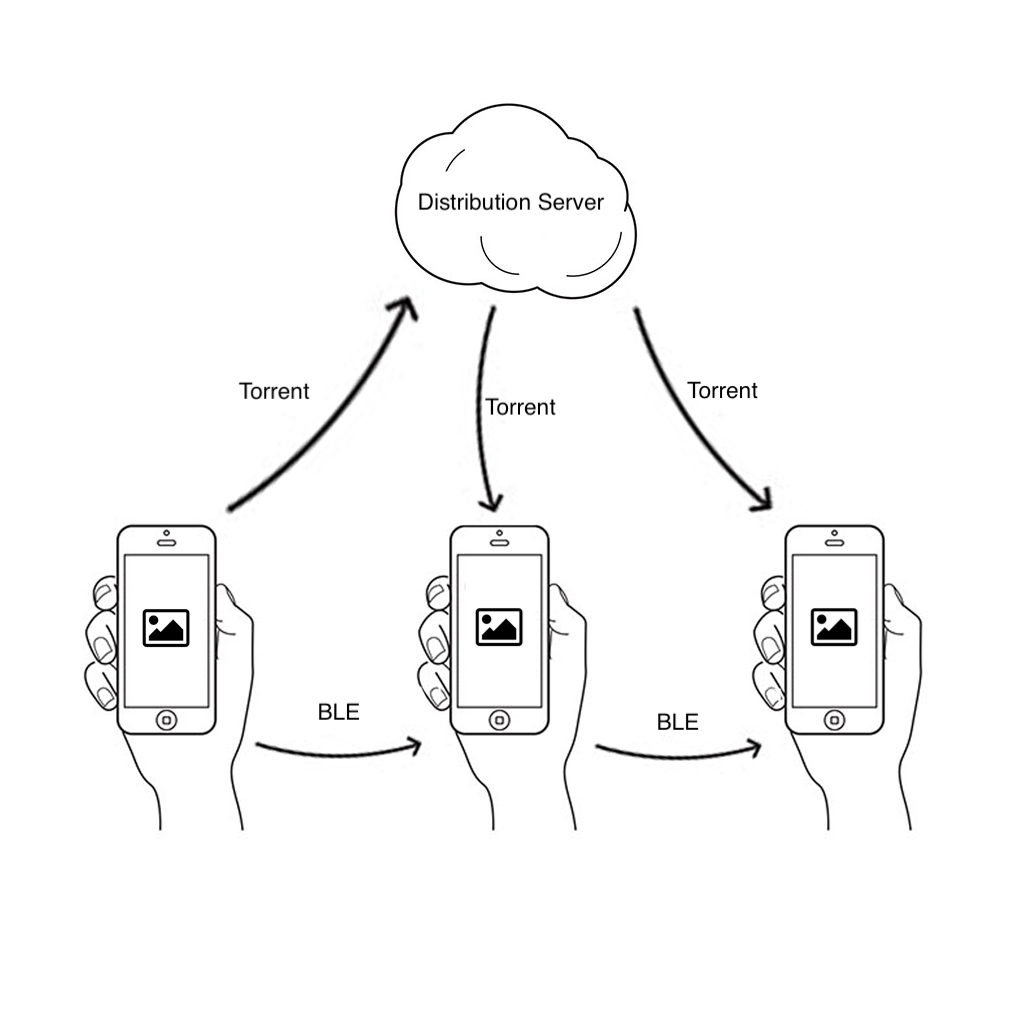
\includegraphics[width=\columnwidth]{overview.jpg}
    \lfig{system-overview}
    \vspace{-5mm} % use negative white space to fix too large gaps
	\caption{System Overview~\cite{estimote}}
\end{figure}

\section{Work Packages}
We identified and sectioned the project in the following work packages: 

\begin{itemize}
    \item {\bf WP1 - BitTorrent Client}: Implementing the management of the embedded BitTorrent Client.
    \item {\bf WP2 - Distribution Server}: Implementing a RESTful API for torrent file distribution.
    \item {\bf WP3 - Camera UI}: Implementing the camera and photo capture functionality of the app using the Android API.
    \item {\bf WP4 - Receive UI}: Implementing the receive stack of Ripples including the reripple and discard functionality.
    \item {\bf WP5 - BLE Sending}: Implementing the sending/broadcasting of Ripples via Bluetooth Low Energy.
    \item {\bf WP6 - BLE Receiving}: Implementing the receiving and scanning of Ripples via Bluetooth Low Energy.
    \item {\bf WP7 - Local Database}: Implementing an interface to a local SQLite database for the storage of send and received Ripples.
\end{itemize}

Each working package is intended to be done by an individual team member. Due to the dependencies of some of the packages it is necessary for certain group members to work together. Since some work packages are more extensive than others, team members are encouraged to help their fellow team mates when done with their own part. In the later stages of the project more and more interaction will be required in order to have a working and coherent application for the final submission. 
 
\section{Milestones}

We plan to uphold the following schedule:
\begin{itemize}
\item  \textbf{24. Nov. 2017}: First working versions of the individual work packages
\item  \textbf{4. Dec. 2017}: Integrated all work packages into one coherent app
\item \textbf{8. Dec. 2017}: Testing application on multiple nodes, identifying bugs and generally debugging the system
\item \textbf{14. Dec. 2017}: Finished presentation and Ripple logo. 
\item \textbf{15. Dec. 2017}: Deadline for submission of presentation slides and project logo.
\item \textbf{16. Dec. 2017}: Finished debugging entire system and fully working version of the app.
\item \textbf{17. Dec. 2017}: Deadline for submission of code.
\item \textbf{18. Dec. 2017}: Presentation and demo of project.
\end{itemize}


\bibliographystyle{abbrv}
\bibliography{report}  % sigproc.bib is the name of the Bibliography in this case
% You must have a proper ".bib" file

%\balancecolumns % GM June 2007

\end{document}
